To benchmark the energy consumption on disk storage, we had to choose between indirect methods or direct methods.

%The Indirect methods consist of estimating the energy base how much time he spent in which state and how much the seeks, reads, and writes, and knowing much which operation costs and how much energy he spent every time he which is every state. With that knowledge, we can estimate how much energy consumption during that time. This approach produces good results, but since all energy is an estimate, this procedure including an error margin on the results.

%The other approach is the direct method by using external hardware, this method consists of measuring Electric Potential Difference on the disk. This method is a lot precise since the results are real, but the downsize it is that have an impact on the overall performance, this impact it only notices on a big scale~\cite{portela2016}.

It was opt-in for a instant power measurement approach because this was the simplest and sufficient solution to achieve the objectives intended of reading, constantly and automatically the energy consumption on the secondary storage ensuring that our results are precise and reliable and since our measurements are on a small scale it doesn't have an impact on the overall systemy~\cite{portela2016}.

Since it is necessary data handling on our behalf and because we need to store energy spent, a normal ammeter won't do the work. Thus to gather our measurements we choose to use an Arduino Uno with a current sensory~\cite{portela2016}.

The SATA cable is responsible for distributing energy to the disk and data exchange between the secondary memory and the computer. So to get the energy on the disk we must connect the current sensor to the connection of the SATA cable that is responsible for distributing energy~\cite{portela2016}.

The current sensor we opt-in was the Low Current Sensor Breakout. This current sensor is marketed by SparkFun and can measure the current regardless of whether the signal is continuous or alternating. The sensor is also accompanied by an operational amplifier phase to control the gain, which can measure lower currents more precisely ~\cite{portela2016}.

\begin{figure}[H]
  \caption{Scheme of connections between Sata cable, current sensor and Arduino used to measurement secondary storage.}
  \centering
  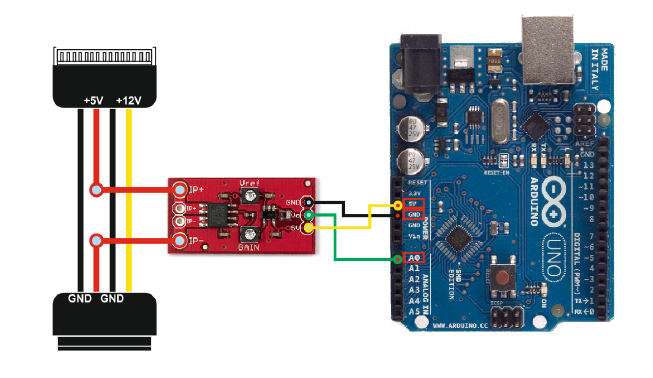
\includegraphics[width=\linewidth]{Chapters/images/arduino.png}
\end{figure}

Also, an Arduino UNO was used to read the analog voltage presented by the sensor and communicate these values to the computer connected to it through the serial port. For this, we had to develop a program for the Arduino that would get take constant readings at the analog voltage and send them every 0.1 seconds. 

  \begin{lstlisting}[ caption={ Arduino source code for reading the analog signal from the current sensor},label={lst:arduinocode},language=C,
    basicstyle=\small
]
void loop() {
  /* Initialization */
  float average_a0 = 0; // Raw reading from pin
  float voltage = 0; // Voltage in V
  float current = 0; // Current in A
  float wattage = 0; // Wattage in W
  float power = 0; // Power in J
  /* Average loop */
  for(int i = 0; i < n_reads ; i++) {
    average_a0 += analogRead(sensorPin_0);
    delay(loop_delay);  }
  /* Formula based computations */
  average_a0 /= n_reads;
  voltage = (average_a0 / 1024.0) * 5;
  current = current_eq(voltage);
  wattage = voltage * current;
  power = wattage * interval;
  Serial.println(power, 3);
  Serial.flush();}

\end{lstlisting}


Following the code on the listing \ref{lst:arduinocode}, the reading is made every millisecond and then is made the average of the last one hundred milliseconds, which is finally sent to the computer system connected to the Arduino.
